\documentclass[a4paper, 12pt]{article}%тип документа

%Русский язык
\renewcommand{\familydefault}{\sfdefault}%шрифт
\usepackage[T2A]{fontenc} %кодировка
\usepackage[utf8]{inputenc} %кодировка исходного кода
\usepackage[english,russian]{babel} %локализация и переносы

%отступы 
\usepackage[left=2cm,right=2cm,top=2cm,bottom=3cm,bindingoffset=0cm]{geometry}
\usepackage{indentfirst}

%Вставка картинок
\usepackage{graphicx}
\usepackage{wrapfig, caption}
\graphicspath{}
\DeclareGraphicsExtensions{.pdf,.png,.jpg, .jpeg}

%Таблицы
\usepackage[table,xcdraw]{xcolor}
\usepackage{booktabs}

%Графики
\usepackage{pgfplots}
\pgfplotsset{compat=1.9}

%Математика
\usepackage{amsmath, amsfonts, amssymb, amsthm, mathtools}

%Заголовок
\author{Нугманов Булат \\ Подлесный Артём}
\title{1.3 \\ Эффект Рамзауэра}
\begin{document}
	\maketitle
	
	\section*{Краткая теория}
	Эффективное сечение реакции --- это величина, характеризующая вероятность перехода системы двух сталкивающихся частиц в результате их рассеяния (упругого или неупругого) в определенное конечное состояние. Сечение $\sigma$ это отношение числа таких переходов $N$ в единицу времени к плотности потока $nv$ рассеиваемых частиц, падающих на мишень, т.е. к числу частиц, попадающих в единицу времени на единичную площадку, перпендикулярную к их скорости.
	
	\begin{equation}
		\sigma = \frac{N}{nv}
	\end{equation}
	
	Эффект Рамзауэра нельзя объяснить с позиций классической теории. С квантовой же точки зрения картина рассеяния выглядит следующим образом. Внутри атома потенциальная энергия налетающего электрона отлична от нуля, скорость электрона меняется, становясь равной $v'$ в соответсвии с законом сохранения энергии:
	\begin{equation}
		E = \frac{mv^2}{2} = \frac{mv'^2}{2} + U
	\end{equation}
	
	а значит, изменяется и длина его волны де Бройля. Таким образом, по отношению к электронной волне атом ведет себя как преломляющая среда с относительным показателем преломления:
	
	\begin{equation}
		n = \frac{\lambda}{\lambda'} = \sqrt{1 - \frac{U}{E}}
	\end{equation}
	
	Решение задачи о рассеянии электрона на сферическом потенциале достаточно громоздко. Поэтому рассмотрим более простое одномерное приближение: электрон рассеивается на потенциальной яме конечной глубины. Уравнение Шрёдингера в этом случае имеет вид:
	\begin{equation}
		\psi'' + k^2\psi = 0 \qquad k^2 = \begin{cases}
			k_1^2  = \frac{2mE}{\hbar^2} \\
			k_2 = \frac{2m(E+U_0)}{\hbar^2}
		\end{cases}
	\end{equation}
	
	Коэффициент прохождения равен отношению квадратов амплитуд прошедшей и падающей волн и определяется выражением:
	\begin{equation}
		D = \frac{16k_1^2k_2^2}{16k_1^2k_2^2 + 4(k_1^2-k_2^2)^2\sin^2(k_2l)}
	\end{equation}
	
	Видно, что коэффициент прохождения частицы над ямой, в зависимости от её энергии, имеет вид чередующихся максимумов и минимумов. В частности, если $k_2l = \pi$, то коэффициент прохождения равен 1, т.е. отраженная волна отсутствует, и электрон беспрепятственно проходит через атом. Этот эффект является квантовым аналогом просветления оптики. Таким образом, коэффициент прохождения электронов максимален при условии:
	\begin{equation}
		k_2l = \sqrt{\frac{2m(E+U_0)}{\hbar^2}}l = \pi n
	\end{equation}
	Прошедшая волна 1 усилится волной 2, если геометрическая разность хода между ними $\Delta = 2l = \lambda'$, что соответствует условию первого интерференционного максимума, т.е.
	\begin{equation}
		2l = \frac{h}{\sqrt{2m(E_1 + U_0)}}
	\end{equation}
	C другой стороны, прошедшая волна ослабится, если $2l = \frac{3}{2}\lambda'$, т.е.
	\begin{equation}
		2l = \frac{3}{2}\frac{h}{\sqrt{2m(E_2+U_0)}}
	\end{equation}
	Решая эти уравнения совместно можно исключить $U_0$ и найти эффективный размер атома $l$:
	\begin{equation}
		l = \frac{h\sqrt{5}}{\sqrt{2m(E_2-E_1)}}
	\end{equation}
	Понятно, что энергии $E_1$, $E_2$ соответсвуют энергия электронов, прошедших разность потенциалов $V_1$ и $V_2$.
	Кроме того, можно оценить эффективную глубину потенциальной ямы атома:
	\begin{equation}
		U_0 =\frac{4}{5}E_2 - \frac{9}{5}E_1
	\end{equation}
	
	Теперь рассмотрим ВАХ тиратрона. Она имеет вид:
	$$
	I_a = I_0e^{-C\omega(V)}, C = Ln_a\Delta_a
	$$
	где $I_0 = eN_0$ --- ток катода, $I_a = eN_a$ --- анодный ток, $\Delta_a$ --- площадь поперечного сечения атома, $n_a$ --- концентрация атомов газа в лампе, $L$ --- расстояние от катода до анода, $\omega(V)$ --- вероятность рассеяния электрона на атоме как функция от ускоряющего напряжения. По измеренной ВАХ тиратрона можно определить зависимость вероятности рассеяния электрона от его энергии из соотношения:
	\begin{equation}
		\omega(V) = -\frac{1}{C}\ln\frac{I_a}{I_0}
	\end{equation}
	\section*{Установка}
	Лампа-тиратрон ТЗ01/1.3Б, заполненная инертным газом, расположена непосредственно на корпусе блока источников питания. Напряжение к электродам лампы подаются от источников питания, находящихся в корпусе прибора. Регулировка напряжения и выбор режима работы установки производится при помощи ручек управления, выведенных на лицевую панель блока источников питания.
	\begin{center}
		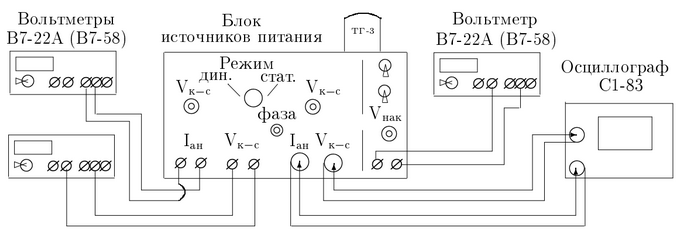
\includegraphics[width=\textwidth]{11.png}
		\textbf{Рис. 1 Схема экспериментальной установки}
	\end{center}
	\section*{Обработка экспериментальных данных}
	\subsection*{Статический метод}
	
	По напряжению пробоя (максимальное напряжение, полученное на установке) определяем $U_{ион.}\approx 11 \text{В}$, значит, что наш газ --- ксенон.
	
	По формулам рассчитаем характерный размер электронной оболочки атома ксенона и глубину потенциальной ямы.
	\begin{equation*}
		l = \frac{h\sqrt{5}}{\sqrt{32m(E_2-E_1)}}
	\end{equation*}
	\begin{equation*}
		U_0 =\frac{4}{5}E_2 - \frac{9}{5}E_1
	\end{equation*}
	\begin{center} 
		\textbf{Таблица 1} \\ 
		\begin{tabular}{|c|c|c|c|c|c|}
			\hline
			\rowcolor[HTML]{C0C0C0}
			& $U_{\text{накала}}, \text{В}$ & $l, \small{\text{Å}}$ & $\Delta l, \small{\text{Å}}$ & $U_0, \text{эВ}$ & $\Delta U_0, \text{эВ}$ \\ \hline
			\cellcolor[HTML]{C0C0C0} 1 & 2.7 & 3.17 & 0.05 & 1.43 & 0.12 \\ \hline
			\rowcolor[HTML]{EFEFEF}
			\cellcolor[HTML]{C0C0C0} 2 & 3.0 & 3.11 & 0.03 & 1.49 & 0.08 \\ \hline
		\end{tabular}
	\end{center}

	Найдём зависимость энергий, соответствующих максимум коэффициента прохождения электронов $E_n = f(E_1, n)$:
	\[E_n = n^2\left(E_1+U_0\right)-U_0 \implies 
	\begin{cases}
		E_2 = 13.79 \pm 0.22 eV \\
		E_3 = 32.9 \pm 0.6 eV
	\end{cases}\] \\ \\
	\newpage
	\begin{center}
		\textbf{Рис.  2}\\
		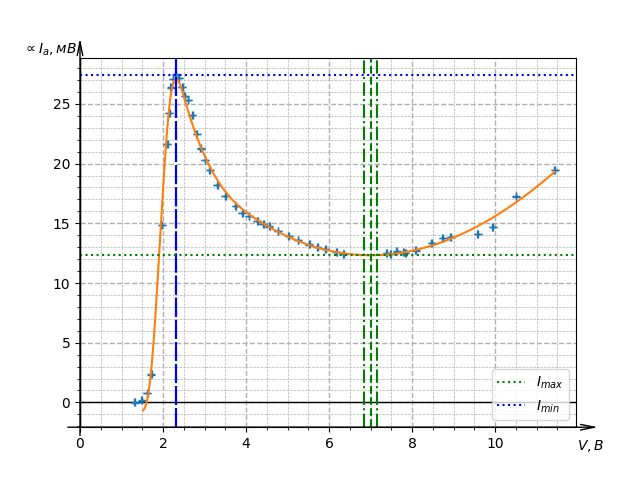
\includegraphics[width=0.75\linewidth]{Figure_1.png}
	\end{center}

	\begin{center}
		\textbf{Рис. 3}\\
		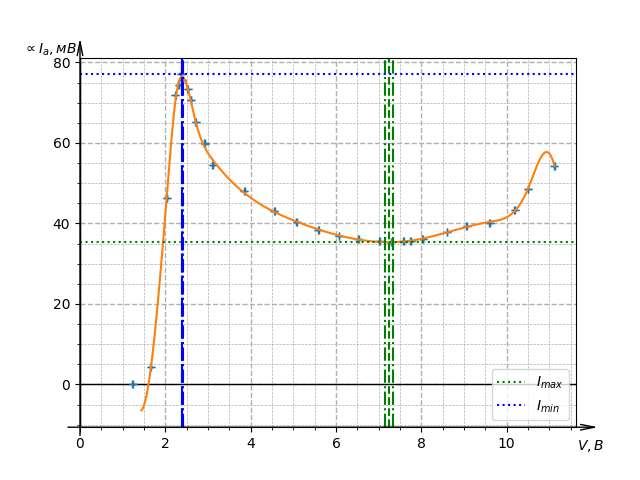
\includegraphics[width=0.75\linewidth]{Figure_2.png}
	\end{center}

	Проведённые рыжие графики проведены не по какой-то формуле, а являются лишь сглаживающими.

	Следующий график показывает лишь качественное поведение, потому что точного значения $C$ и $I_0$. 
	\newpage
	\begin{center}
		\textbf{Рис. 4} Качественный график вероятности прохождения\\
		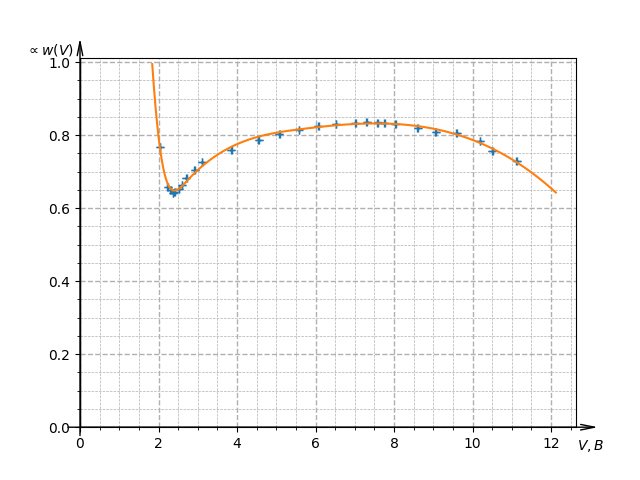
\includegraphics[width=\linewidth]{w.png}
	\end{center}
	\subsection*{Динамический метод}
	Измерение динамическим методом проводятся с помощью осциллографа в пространственном режиме. Тогда на экране осциллографа будет показана ВАХ тиратрона. Измерения проводились при напряжении накала в 2.7 и 3 В. ВАХ показаны на рис.5.
\begin{figure}[h]
\textbf{Рис. 5} ВАХ тиратрона. Как видно, положения максимумов и минимумов не слишком отличаются для прямого и обратного смещения. Масштаб по Х -- 5В.\\
\begin{minipage}[h]{0.43\linewidth}
\center{(2.7 B) \\ 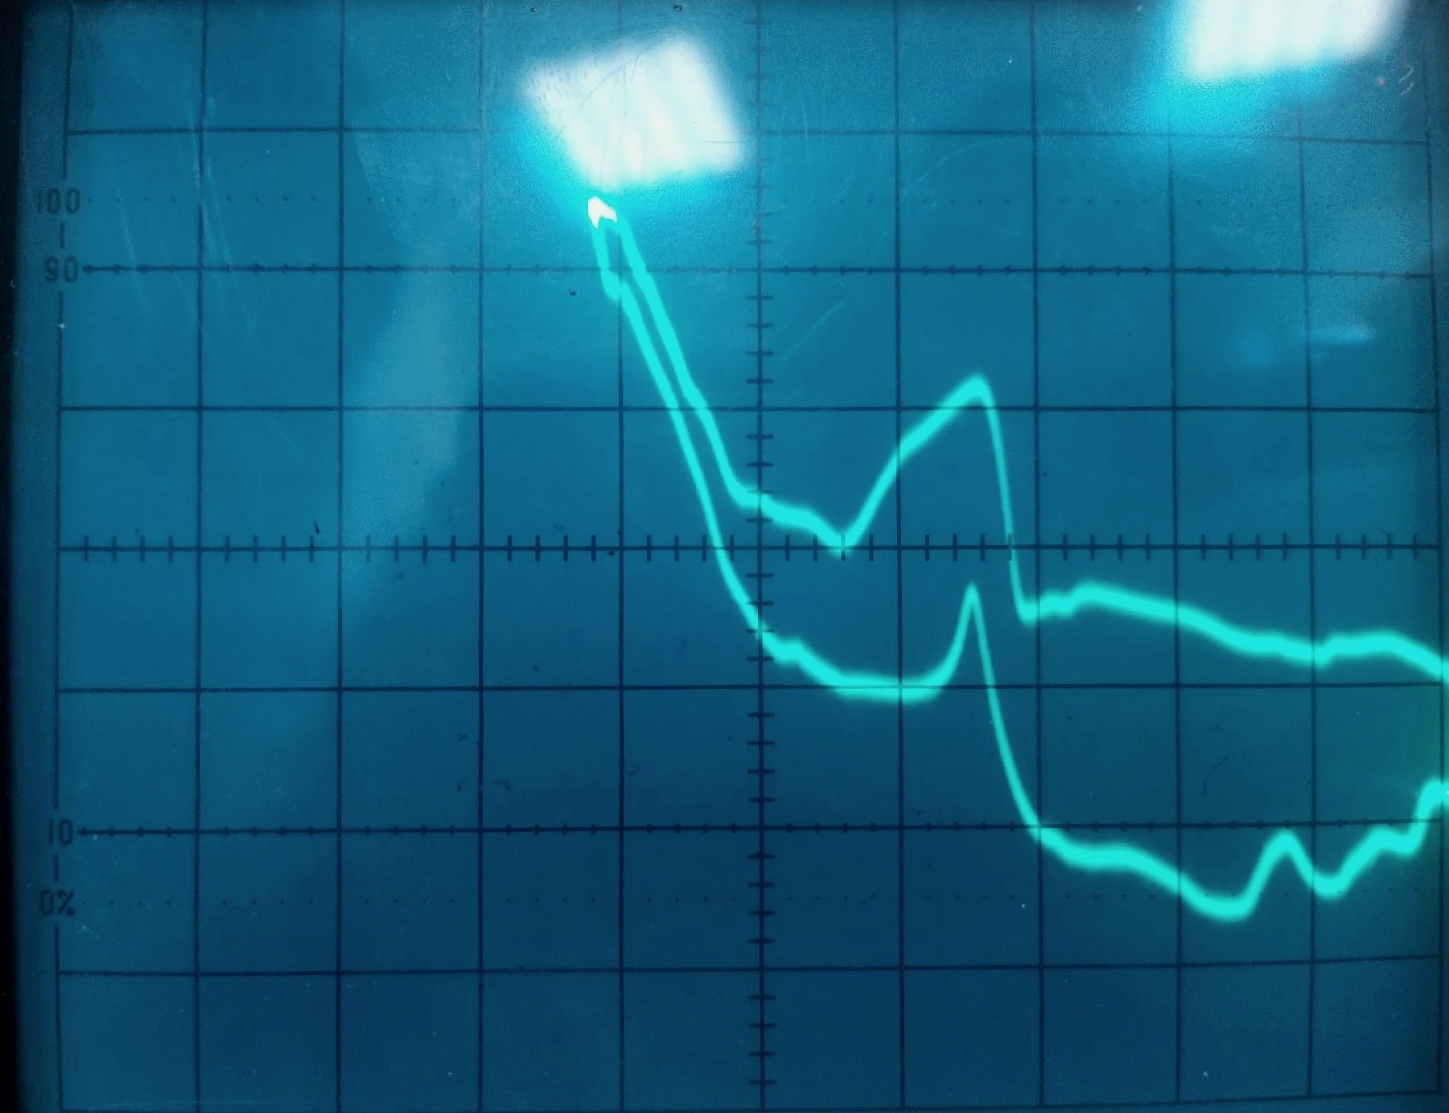
\includegraphics[width=1\linewidth]{dyn27.jpg}}
\end{minipage}
\hfill
\begin{minipage}[h]{0.43\linewidth}
\center{(3 B) \\ 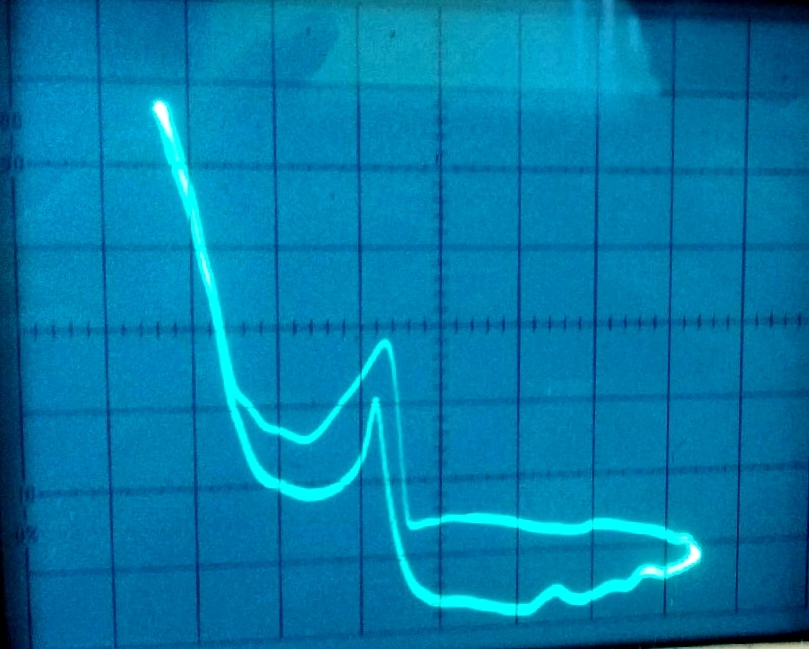
\includegraphics[width=1\linewidth]{dyn3.jpg}}
\end{minipage}
\end{figure}
\newpage
	С помощью ВАХ и предыдущих формул (9), (10) получаем результаты в виде таблицы 2. Напряжение пробоя $U \approx 11 B$, что соответствует результатам статического метода.
	
\begin{center}
\textbf{Таблица 2}\\
\begin{tabular}{|c|c|c|c|c|}
\hline
\rowcolor[HTML]{9B9B9B} 
$V_{\text{накала}}$, B      & $l$, $A$ & $\Delta l$, $A$ & $U_0$, эB & $\Delta U_0$, эB \\ \hline
\cellcolor[HTML]{9B9B9B}2.7 & 3.1        & 0.4               & 2         & 0.52             \\ \hline
\rowcolor[HTML]{EFEFEF} 
\cellcolor[HTML]{9B9B9B}3   & 3.1        & 0.2               & 2.24      & 0.28             \\ \hline
\end{tabular}
\end{center}
	
	
	
	
	
	
	
	
	
	
	
	
	
	
	
	
	
	
	
	
	
	
	
	
	
	
	
	
	
	\section*{Вывод}
	В проделанной работе было изучено явление рассеяния электронов на атомах ксенона. Экспериментальные данные подтверждают гипотезу о волновых свойствах электрона. Были оценены размеры электронной оболочки ксенона и глубина потенциальной ямы атома. Результаты статического и динамического методов равны в пределах погрешности, что свидетельствует о достоверности измерений. Имеющиеся отличия вызваны в основном большой погрешностью в определении положений максимума и минимума на ВАХ с помощью осциллографа. Это общий тренд всех таких работ этого семестра -- динамический метод имеет значительно меньшую достоверность и точность.
	\begin{table}[]
	\begin{tabular}{|c|c|c|c|}
		\hline
		\rowcolor[HTML]{EFEFEF} 
		\multicolumn{2}{|c|}{\cellcolor[HTML]{EFEFEF}$U_{\text{накала}}$=2.7В} & \multicolumn{2}{c|}{\cellcolor[HTML]{EFEFEF}$U_{\text{накала}}$=3В} \\ \hline
		\rowcolor[HTML]{C0C0C0} 
		$I_a$, мВ                           & $V$, В                           & $I_a$, мВ                          & $V$, В                         \\ \hline
		0                                   & 1.32                             & 0                                  & 1.24                           \\ \hline
		0.17                                & 1.49                             & 4.38                               & 1.66                           \\ \hline
		0.8                                 & 1.62                             & 46.26                              & 2.04                           \\ \hline
		2.34                                & 1.72                             & 65.24                              & 2.71                           \\ \hline
		14.84                               & 1.97                             & 54.58                              & 3.11                           \\ \hline
		24.26                               & 2.15                             & 59.87                              & 2.92                           \\ \hline
		27.2                                & 2.38                             & 70.63                              & 2.6                            \\ \hline
		25.63                               & 2.52                             & 73.41                              & 2.52                           \\ \hline
		26.44                               & 2.46                             & 75.7                               & 2.4                            \\ \hline
		27.46                               & 2.31                             & 74.44                              & 2.31                           \\ \hline
		21.61                               & 2.1                              & 71.9                               & 2.23                           \\ \hline
		27.07                               & 2.24                             & 77.03                              & 2.37                           \\ \hline
		26.38                               & 2.18                             & 48                                 & 3.85                           \\ \hline
		25.34                               & 2.6                              & 43.11                              & 4.55                           \\ \hline
		24.06                               & 2.7                              & 40.3                               & 5.08                           \\ \hline
		22.47                               & 2.81                             & 38.35                              & 5.58                           \\ \hline
		21.27                               & 2.91                             & 36.9                               & 6.07                           \\ \hline
		20.3                                & 3.01                             & 36.14                              & 6.52                           \\ \hline
		19.47                               & 3.12                             & 35.58                              & 7.01                           \\ \hline
		18.21                               & 3.31                             & 35.52                              & 7.58                           \\ \hline
		17.26                               & 3.5                              & 36.15                              & 8.03                           \\ \hline
		16.44                               & 3.75                             & 35.6                               & 7.75                           \\ \hline
		15.89                               & 3.91                             & 35.28                              & 7.3                            \\ \hline
		15.6                                & 4.07                             & 37.89                              & 8.6                            \\ \hline
		15.2                                & 4.27                             & 39.39                              & 9.06                           \\ \hline
		14.95                               & 4.41                             & 40.01                              & 9.6                            \\ \hline
		14.74                               & 4.56                             & 43.27                              & 10.19                          \\ \hline
		14.34                               & 4.77                             & 48.6                               & 10.5                           \\ \hline
		13.96                               & 5.03                             & 54.31                              & 11.12                          \\ \hline
		13.63                               & 5.25                             &                                    &                                \\ \hline
		13.23                               & 5.52                             &                                    &                                \\ \hline
		13.04                               & 5.72                             &                                    &                                \\ \hline
		12.84                               & 5.91                             &                                    &                                \\ \hline
		12.61                               & 6.17                             &                                    &                                \\ \hline
		12.46                               & 6.35                             &                                    &                                \\ \hline
		12.52                               & 7.39                             &                                    &                                \\ \hline
		12.53                               & 7.83                             &                                    &                                \\ \hline
		12.42                               & 7.47                             &                                    &                                \\ \hline
		12.73                               & 8.09                             &                                    &                                \\ \hline
		12.58                               & 7.8                              &                                    &                                \\ \hline
		12.64                               & 7.63                             &                                    &                                \\ \hline
		13.35                               & 8.47                             &                                    &                                \\ \hline
		13.87                               & 8.93                             &                                    &                                \\ \hline
		13.77                               & 8.74                             &                                    &                                \\ \hline
		14.08                               & 9.58                             &                                    &                                \\ \hline
		14.67                               & 9.94                             &                                    &                                \\ \hline
		17.25                               & 10.5                             &                                    &                                \\ \hline
		19.47                               & 11.43                            &                                    &                                \\ \hline
	\end{tabular}
\end{table}
\end{document}